\subsection{Modeling Setup, Boundary Conditions, and Coupling}\label{sec:cfd-dem-setup}
For this simulation, I begin with the same well-packed pebble bed set up in \cref{sec:dem-studies-effective-conductivity}. I will analyze a full-packed bed and a damaged bed with $\eta = 10$\% of broken pebbles. The random removal technique of inducing `damage' to the bed was again used (in the same manner as described in \cref{sec:dem-studies-effective-conductivity}). The intent is to deduce changes in thermophysical properties when helium is considered in the thermal transport network of the pebble bed -- and as a function of the morphological changes due to damaged pebbles.

The domain of the pebble bed in this study is a clone of the DEM study done previously. The fluid domain is constructed to include an inlet and outlet region of fluid to permit development of the flow profiles. The inlet region is 5 pebble diameters in length and the outlet is 30 pebble diameters. No-slip boundary conditions are enforced at the walls at the $x$-limits of the region. To match the DEM domain, periodic boundary conditions are used in the $y$-limits. The inlet face of the fluid is specified at a constant $\vec{v} = (5, 0, 0)$ \si{\centi\meter\per\second}. The outlet face is specified with OpenFOAM's `inletOutlet' command with a given pressure. This boundary condition allows the inlet pressure to float to value that satisfies the specified inlet velocity and outlet pressure. The temperature is specified as a constant $T_w = $ \SI{573}{\kelvin} at the $x$-walls as well as the inlet. The outlet condition of the temperature field is similarly given to be `inletOutlet' with OpenFOAM.

The size of the CFD cells were chosen to be large enough to fit approximately 5 pebbles, for which the divided technique of computing void fraction is applicable (see \cref{sec:lag-eul-mapping}); the ratio of cell volume to particle volume was $V_\text{cell} / V_p = 7.46$. The helium, in this first model, was modeled with constant fluid properties. The values are given in Table~\ref{tab:cfd-properties}.

The Koch-Hill-Ladd drag model is employed in the style of Model B with an Archimedes pressure for buoyancy term. The terminology of these CFD coupling drag models is discussed in Ref.~\cite{Zhou2010} The Nusselt number correlation of Li \& Mason is used for calculating the Nusselt number. OpenFOAM's dummy turbulence model (which is nothing more than a laminar model) is used.

An implicit time marching scheme is employed with a time step in the fluid domain of $\Delta t_f =$\SI{1e-4}{\second}. The small time step is not necessary to capture the fluid flow. The momentum equation is essentially not even transient as a steady-state laminar solution is achieved almost instantaneously in comparison to the long time span required to reach thermal steady state. The small time step is necessary for a relatively tight coupling to the pebble bed as the temperatures increase on the pebbles. Integration schemes of gradients, divergence terms, and laplacians are all Gauss linear or Gauss limitedLinear (as defined in OpenFOAM). The time step of the DEM is $\Delta t_s =$ \SI{1e-7}{\second} which must be small for stability of the DEM explicit integration. The coupling between CFD and DEM domains occurs every 10 time steps of the fluid domain - equating to every \num{10000} in the pebble domain.

The layout of the pebble bed inside the CFD domain is shown in Figs.~\ref{fig:cfdem-domain-x}, \ref{fig:cfdem-domain-y}, and~\ref{fig:cfdem-domain-z}. Notable of the layout is the relaxation of the mesh size in the direction of the periodic boundaries. The size is permitted as there are few variations in fluid or temperature in the periodic direction. The meshes are made much smaller in the direction between cooling boundaries. In this direction ($x$-direction), we need the meshes small enough to resolve a temperature and velocity profiles across the bed between centerline and cooling boundaries. We also want to capture the behavior of near-wall arrangement of the pebble bed. 

\begin {table}[htp] %
\caption{Constant fluid properties of helium purge gas in CFD-DEM coupling.}
\label {tab:cfd-properties} \centering %
\begin {tabular}{ ccccc }
\toprule %
$\nu$				&	$\alpha$				&	$k$		&	$C_p$		& $\rho$		\\
(\si{\meter\squared\per\second})			&	(\si{\meter\squared\per\second})				&	(\si{\watt\per\meter\per\kelvin})	&	(\si{\joule\per\kilogram\per\kelvin})	& (\si{\kilogram\per\cubic\meter})	\\\toprule
\num{4.02e-4} &	\num{6.06e-4}	& 	\num{0.2}		& 	\num{5192.8}		& 	\num{0.175}		\\\bottomrule
\end{tabular}
\end{table}


\begin{figure}[t]
	\centering
	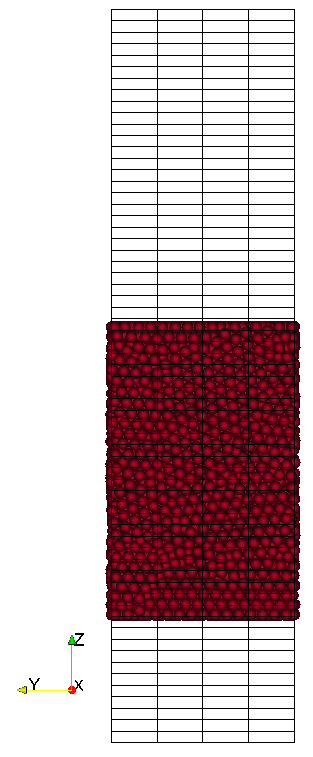
\includegraphics[width=0.4\textwidth]{chapters/figures/x-side-view}
    \caption{Side view of the pebble bed as it resides in the CFD mesh. The meshes in the direction of the periodic faces are allowed to be larger than others.}\label{fig:cfdem-domain-x}
\end{figure}

\begin{figure}[t]
	\centering
	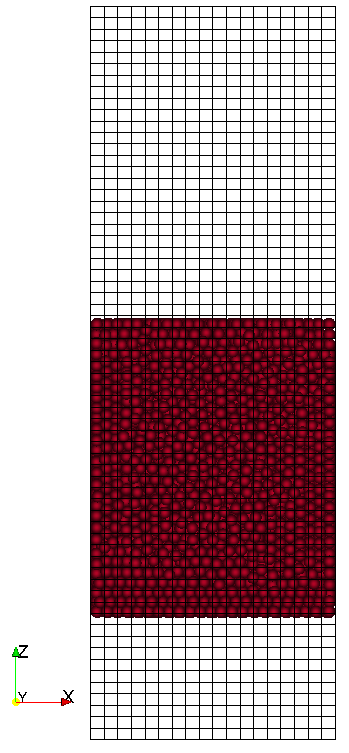
\includegraphics[width=0.4\textwidth]{chapters/figures/y-side-view}
    \caption{Front view of the pebble bed as it resides in the CFD mesh. The meshes in the direction of cooling are chosen to be large enough to fit many pebbles but small enough to provide a resolved temperature profile.}\label{fig:cfdem-domain-y}
\end{figure}

\begin{figure}[t]
	\centering
	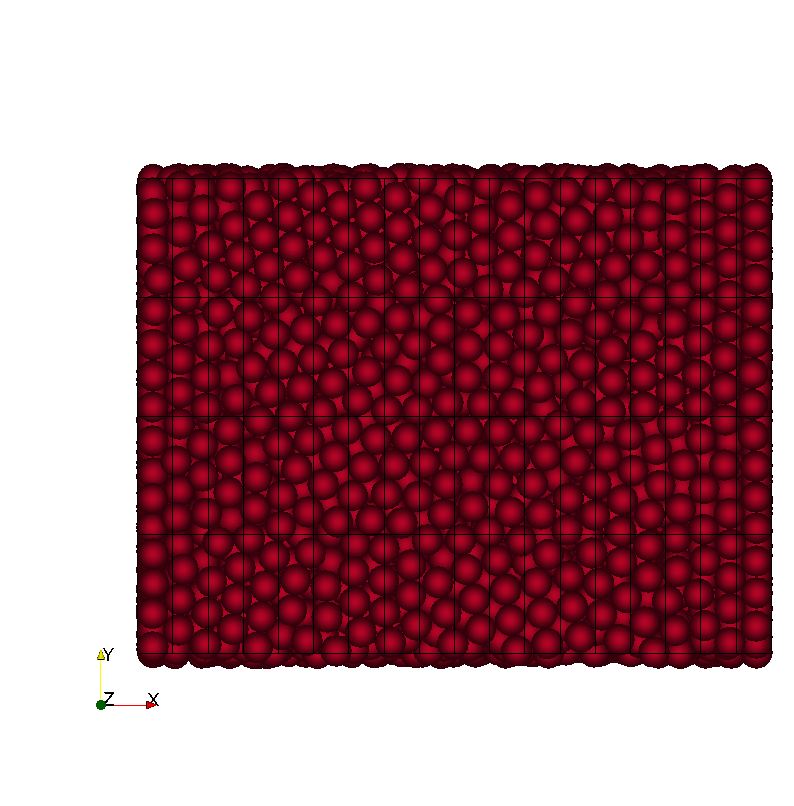
\includegraphics[width=\singleimagewidth]{chapters/figures/z-top-view}
    \caption{Top view of the pebble bed as it resides in the CFD mesh.}\label{fig:cfdem-domain-z}
\end{figure}


While the energy transport is the main concern of the pebble bed, I perform a simple validation of the CFD-DEM routine against known pressure-drop correlations to provide confidence in the overall coupling and volume-averaging technique. After pressure drop is shown to be consistent with empirical predictions, I proceed with the thermal analysis.
\FloatBarrier